\subsection{Apparato}
%
    \begin{figure}[H]
    \centering
    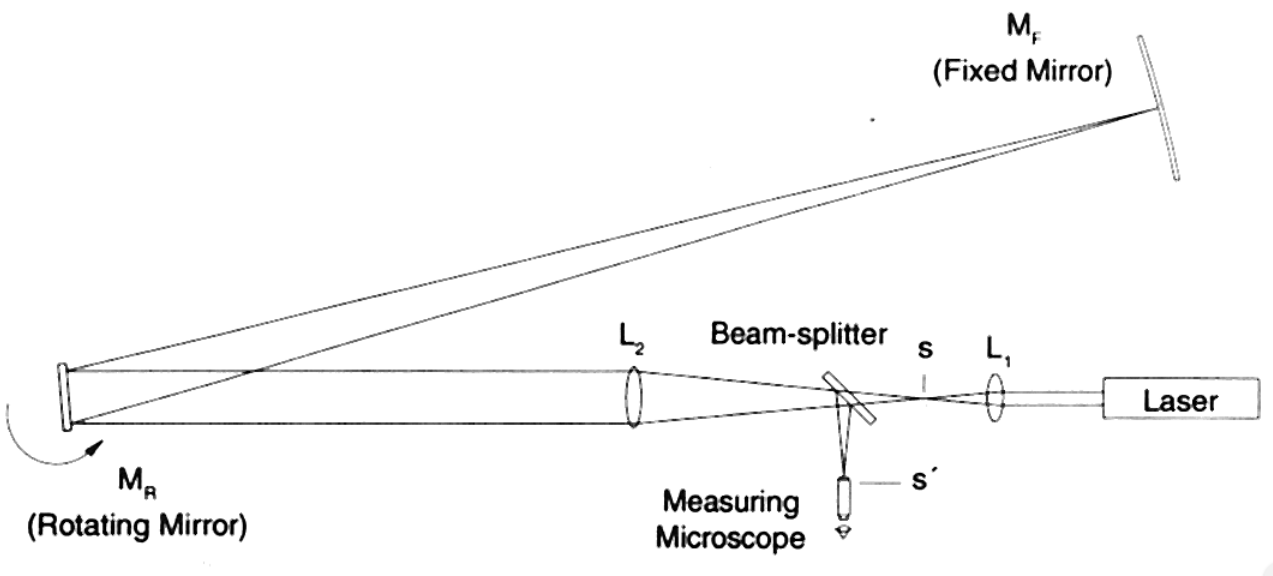
\includegraphics[scale=.3]{Grafici/O1_apparatus.png}
    \caption{Apparato sperimentale}
    \end{figure} 
%
I raggi paralleli all'asse ottico prodotti da una sorgente laser vengono focalizzati in un punto $s$ da una prima lente convergente $L1$.\\\\
%
Prima della seconda lente $L2$ uno specchio semiriflettente convoglia una parte del segnale ottico ad un microscopio, utilizzato per la lettura della misura.\\\\
%
La seconda lente $L2$, avente una distanza focale molto maggiore della prima lente $L1$ ma comunque inferiore alla distanza che la separa dal punto $s$, focalizza i raggi ad una distanza $ p>f2>f1 $.\\\\
%
\textcolor{red}{Prima del punto $A$ si trova interposto uno specchio imperniato su un supporto rotante che direziona i raggi verso uno specchio sferico di raggio $\sim A$; ciò fa sì che i raggi riflessi dallo specchio sferico ritornino sempre allo specchio rotante.}
COSA È IL PUNTO A?? VEDERE SCHEMA DI ALFREDO